\chapter{Results (15 pgs)}

\section{Drag force graphs}

Fundamental:

\begin{figure}[h]
	\centering
	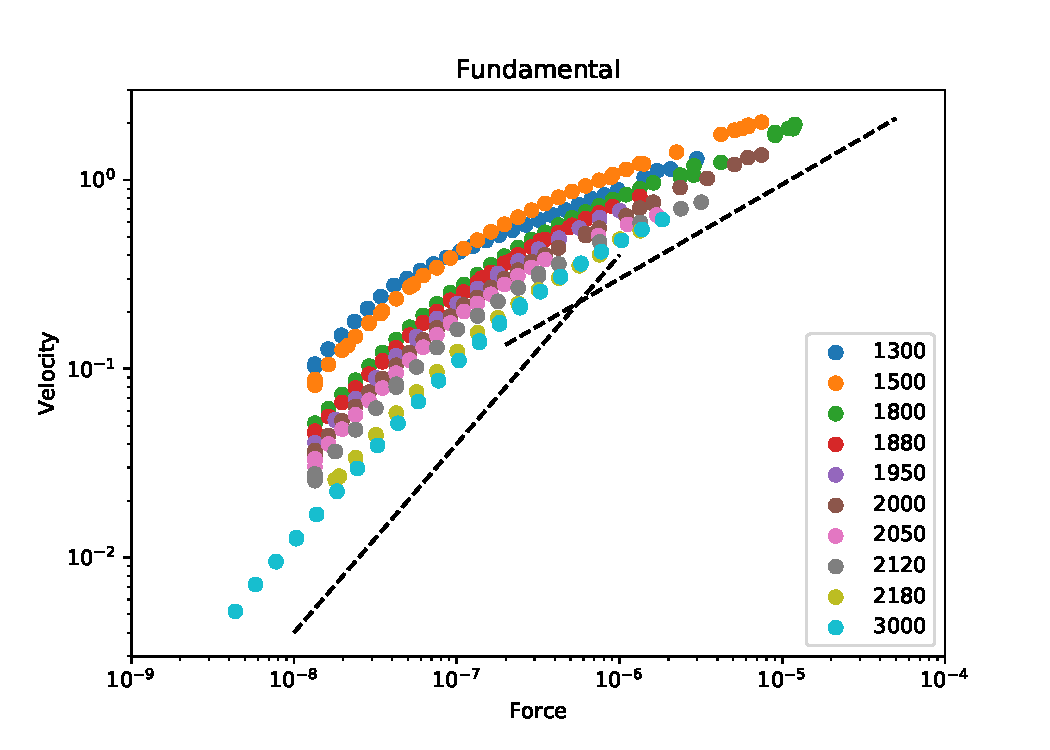
\includegraphics[width=0.8\textwidth]{graphics/results/fund-force_vel}
	\caption{Velocity against force}
	\label{fund_vel_force}
\end{figure}

Overtone:

\begin{figure}[h]
	\centering
	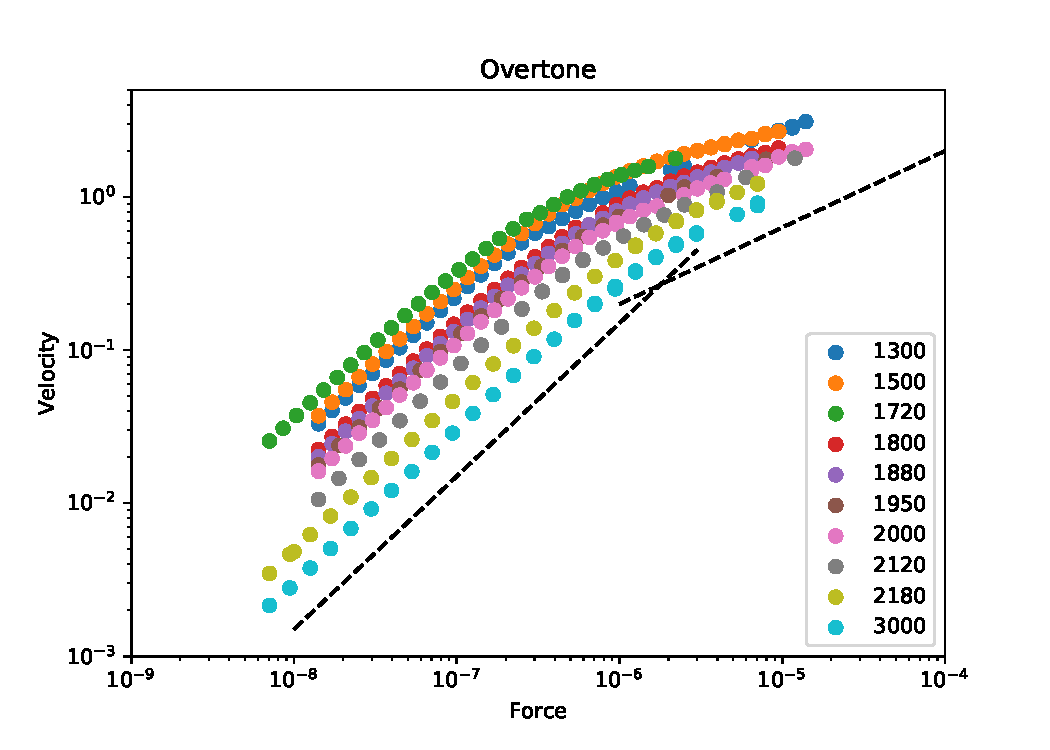
\includegraphics[width=0.8\textwidth]{graphics/results/over-force_vel}
	\caption{Velocity against force}
	\label{over_vel_force}
\end{figure}

Fundamental drag coefficient:

\begin{figure}[h]
	\centering
	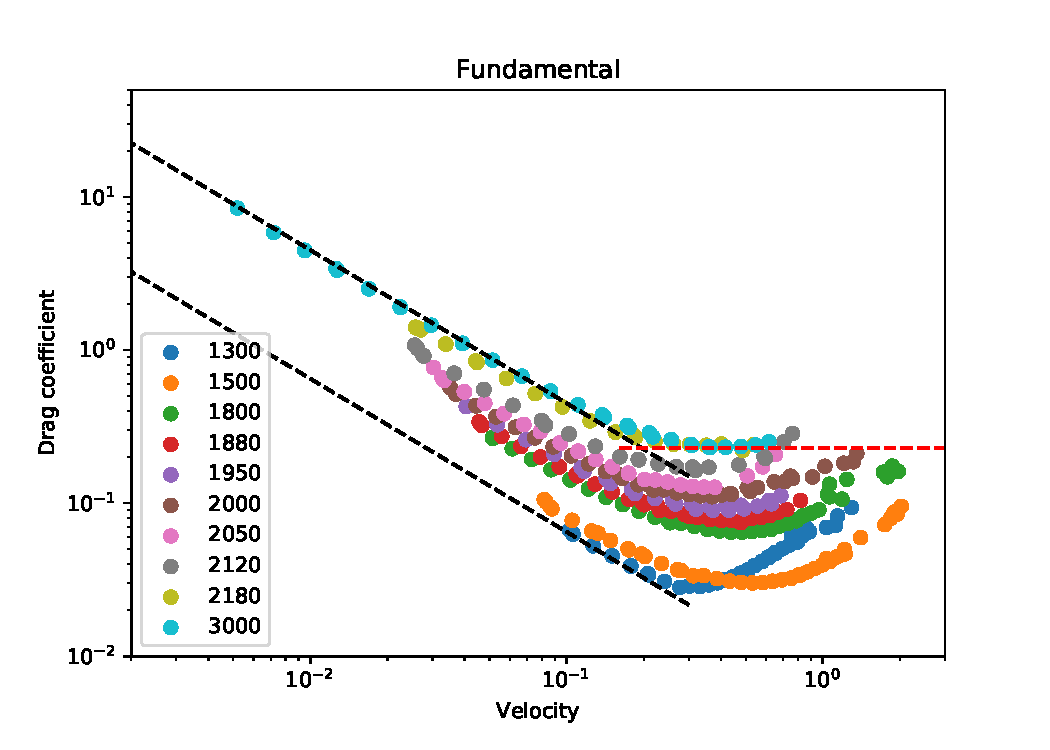
\includegraphics[width=0.8\textwidth]{graphics/results/fund-coeff_vel}
	\caption{Drag coeff against velocity}
	\label{fund_drag_vel}
\end{figure}

Overtone drag coefficient:

\begin{figure}[h]
	\centering
	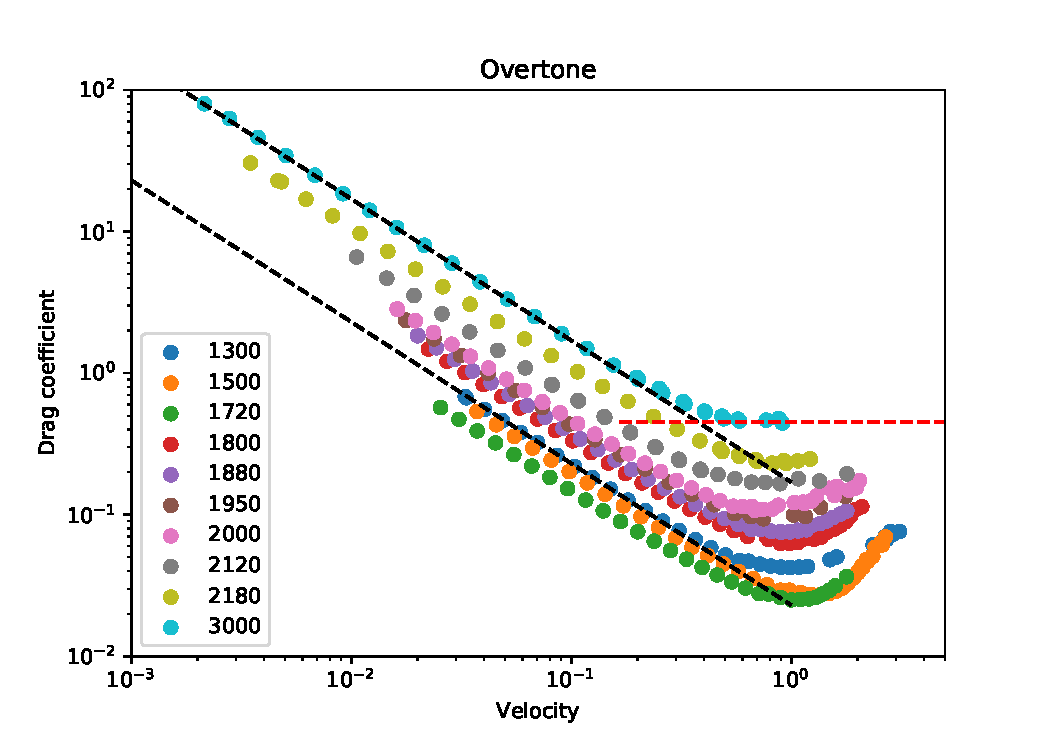
\includegraphics[width=0.8\textwidth]{graphics/results/over-coeff_vel}
	\caption{Drag coeff against velocity}
	\label{fund_drag_vel}
\end{figure}

\section{Universal Scaling}

Fundamental Donnelly:

\begin{figure}[h]
	\centering
	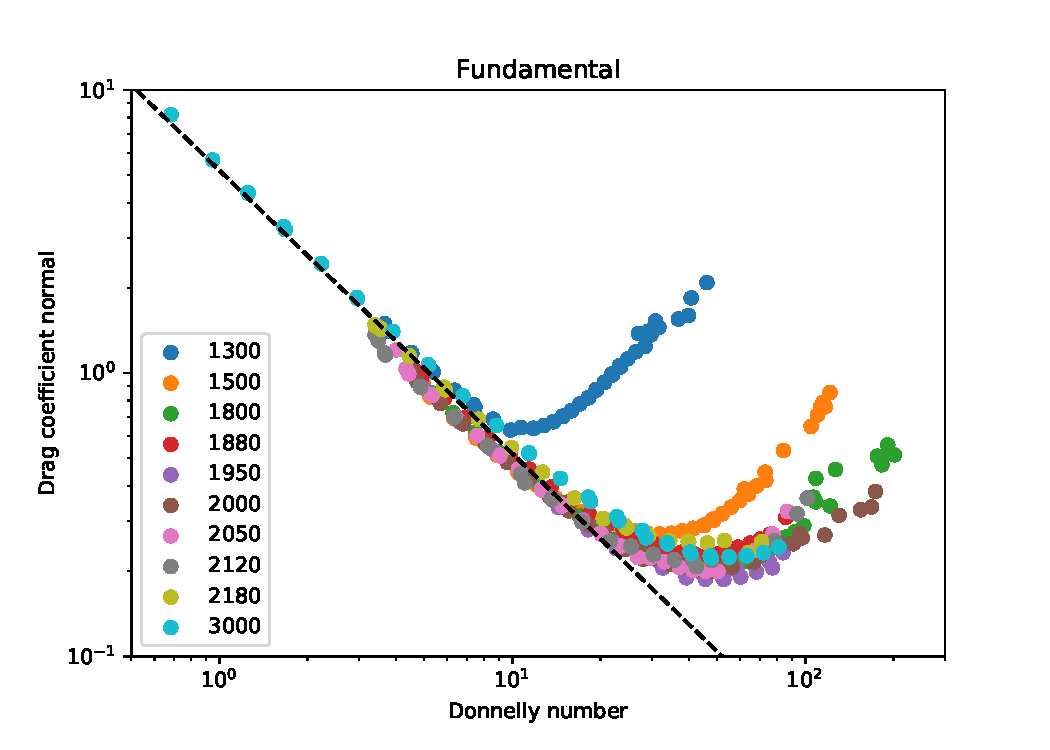
\includegraphics[width=0.8\textwidth]{graphics/results/fund-donnelly}
	\caption{Donnelly num against velocity}
	\label{fund_donnelly}
\end{figure}

Overtone Donnelly:

\begin{figure}[h]
	\centering
	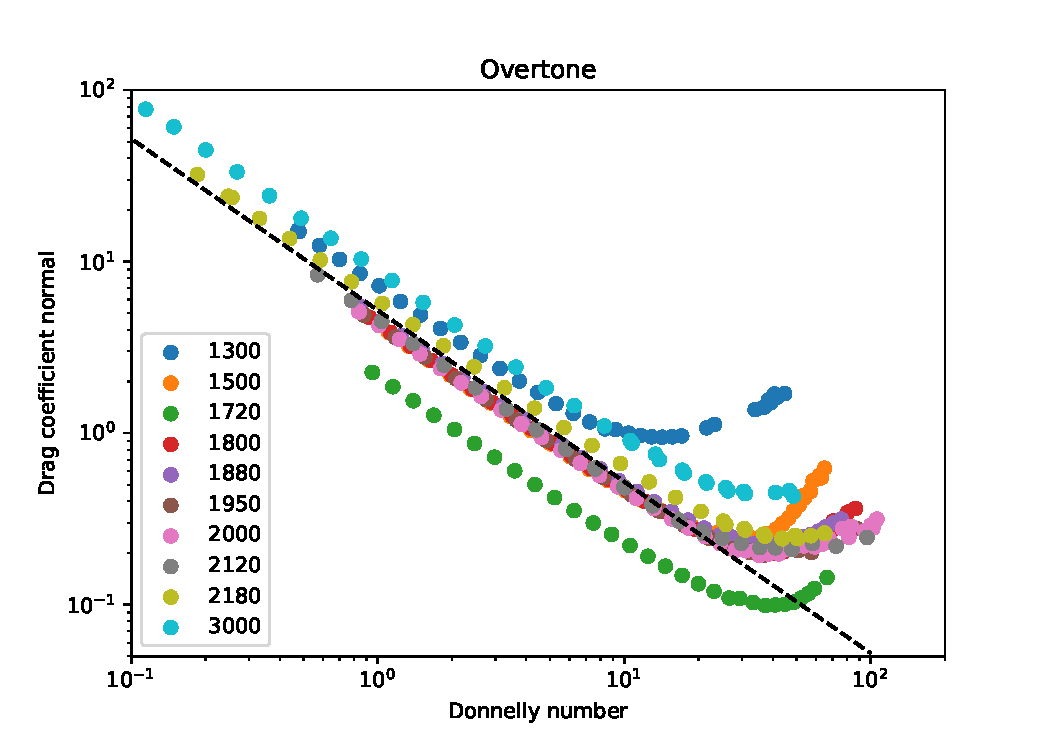
\includegraphics[width=0.8\textwidth]{graphics/results/over-donnelly}
	\caption{Donnelly num against velocity}
	\label{over_donnelly}
\end{figure}

\section{Flow phase diagram}

Fundamental phase diagram:

\begin{figure}[h]
	\centering
	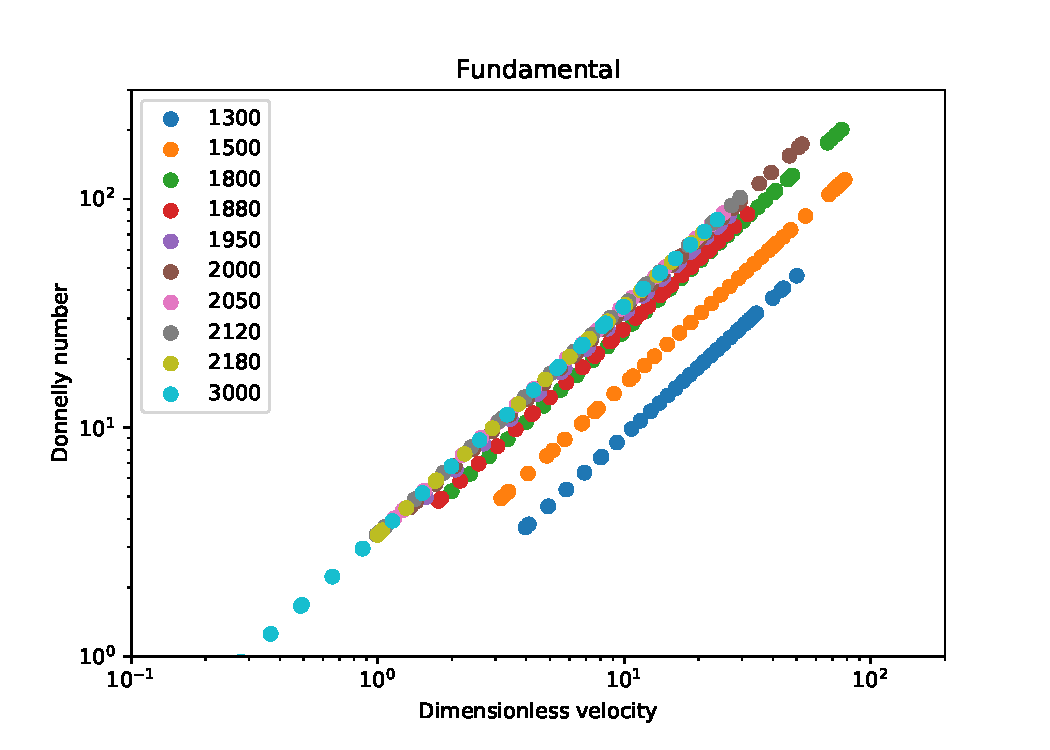
\includegraphics[width=0.8\textwidth]{graphics/results/fund-phase}
	\caption{Donnelly num against dimless velocity}
	\label{fund_phase}
\end{figure}

Overtone phase diagram:

\begin{figure}[h]
	\centering
	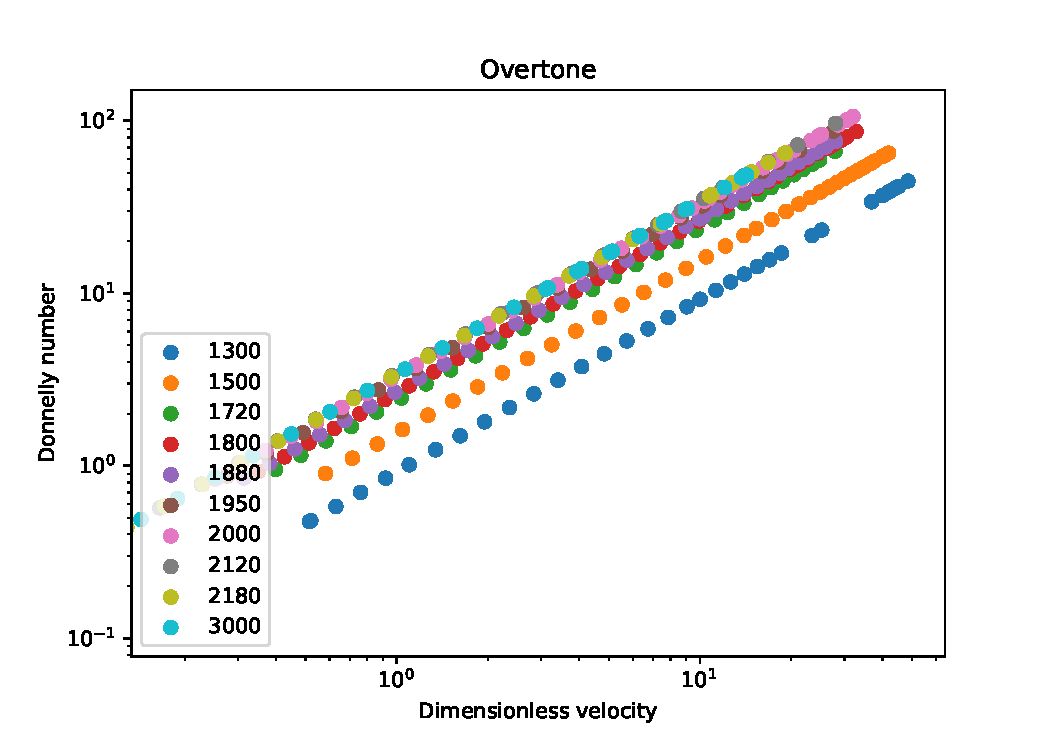
\includegraphics[width=0.8\textwidth]{graphics/results/over-phase}
	\caption{Donnelly num against dimless velocity}
	\label{over_phase}
\end{figure}


\newpage
